\clearpage
\phantomsection

\setcounter{chapter}{0}
\chapter[TỔNG QUAN VỀ CÁC PHƯƠNG PHÁP NHẬN DẠNG HỆ THỐNG TRONG TRUYỀN THÔNG KHÔNG DÂY]{Tổng quan về các phương pháp nhận dạng hệ thống trong truyền thông không dây}
\label{sec:back}

Việc nhận dạng hệ thống trong truyền thông không dây đã luôn được phát triển ngay từ những thế hệ mạng không dây đầu tiên~\cite{Tse2005}. Ngày nay, các thuật toán ước lượng kênh truyền không dây đã đạt được các bước tiến đánh kể về độ chính xác và dựa trên đặc điểm của các thuật toán có thể chia thành bốn hướng tiếp cận chính như trên hình~\ref{fig:classify}. Bao gồm phương pháp không mù (Non-blind), mù (B), bán mù (SB), và dựa trên học máy, học sâu (AI-based)~\cite{vilas2022}. 
Với mỗi phương pháp, rất nhiều thuật toán đã được đề xuất và cho hiệu quả trong các tình huống cụ thể như các trích dẫn trên hình~\ref{fig:classify}.
Từ cách phân loại kể trên, chương đầu tiên sẽ đưa ra mô hình hệ thống MIMO/mMIMO sử dụng cho luận văn, sau đó sẽ trình bày đôi nét cơ bản về các phương pháp ước lượng kênh truyền này, trong số đó, một số thuật toán được dùng để so sánh kết quả trong các chương sau của luận văn sẽ được trình bày chi tiết.

\begin{figure}[H]
    \centering
    \begin{tikzpicture}
        \node (b1) [startstop] at (0, 0) {Các phương pháp nhận dạng kênh truyền không dây};

        \node (b21) [process, align=center] at (-60mm, -25mm) {Phương pháp không mù};

        \node (b22) [process, align=center] at (-20mm, -25mm) {Phương pháp mù};

        \node (b23) [process, align=center] at (20mm, -25mm) {Phương pháp bán mù};

        \node (b24) [process, align=center] at (60mm, -25mm) {Học máy/Học sâu};

        \node (b31) [below=8mm of b21, process, align=left, fill=green!10!white] {
        - Sử dụng dữ liệu \\
        \hspace{0.1cm} + Dựa trên đào tạo~\cite{Singh2019} \\
        \hspace{0.1cm} + Dựa trên Pilot \\
        \hspace{0.3cm} * ZF~\cite{Jiang2011} \\
        \hspace{0.3cm} * MMSE~\cite{Jiang2011} \\
        \hspace{0.3cm} * Maximum \\ 
        \hspace{0.3cm} Likelihood~\cite{ljung1999system} \\
        - Hướng quyết định~\cite{Ozdemir2007} \\
        \hspace{0.1cm} + Quyết định cứng \\
        \hspace{0.1cm} + Quyết định mềm 
        };

        \node (b32) [below=8mm of b22, process, align=left, fill=green!10!white] {
            - Xác định \\
            \hspace{0.3cm} * {\color{red} MRE}~\cite{original} \\
            \hspace{0.3cm} * CMA~\cite{Treichler1983} \\
            \hspace{0.3cm} * MLE~\cite{abed1997} \\
            - Tính thống kê \\
            \hspace{0.1cm} + Bậc hai~\cite{Tong1994} \\
            \hspace{0.1cm} + Bậc cao~\cite{abed1997}
        };

        \node (b33) [below=8mm of b23, process, align=left, fill=green!10!white] {
            - {\color{red} Sử dụng một phần} \\
            {\color{red}dữ liệu}~\cite{Rekik2021, Ladaycia2017, Ladaycia2019} \\
            - Sử dụng DoA/ \\
            DoD~\cite{Wang2016} \\
            - Sử dụng vị trí~\cite{Lin2020}
        };

        \node (b34) [below=8mm of b24, process, align=left, fill=green!10!white] {
            - Học cổ điển \\
            \hspace{0.3cm} * Hồi quy~\cite{Simeon2022} \\
            - Mạng nơ-ron \\
            \hspace{0.3cm} * {\color{red} DetNet}~\cite{Samuel2019} \\
            - Học tăng cường \\
            \hspace{0.3cm} * Q-learning~\cite{Oh2021}
        };

        \draw[line] (b1.south) -- ([yshift=-5mm]b1.south);
        \draw[arrow] ([yshift=-5mm]b1.south) -| (b21);
        \draw[arrow] ([yshift=-5mm]b1.south) -| (b22);
        \draw[arrow] ([yshift=-5mm]b1.south) -| (b23.north);
        \draw[arrow] ([yshift=-5mm]b1.south) -| (b24.north);

        \draw[arrow] (b21) -- (b31);
        \draw[arrow] (b22) -- (b32);
        \draw[arrow] (b23) -- (b33);
        \draw[arrow] (b24) -- (b34);
        
    \end{tikzpicture}
    \caption{Phân loại các phương pháp ước lượng kênh truyền viễn thông.}
    \label{fig:classify}
\end{figure}

\section{Mô hình hệ thống MIMO/mMIMO}\label{sec:sm}

\begin{figure}[ht]
    \centering
    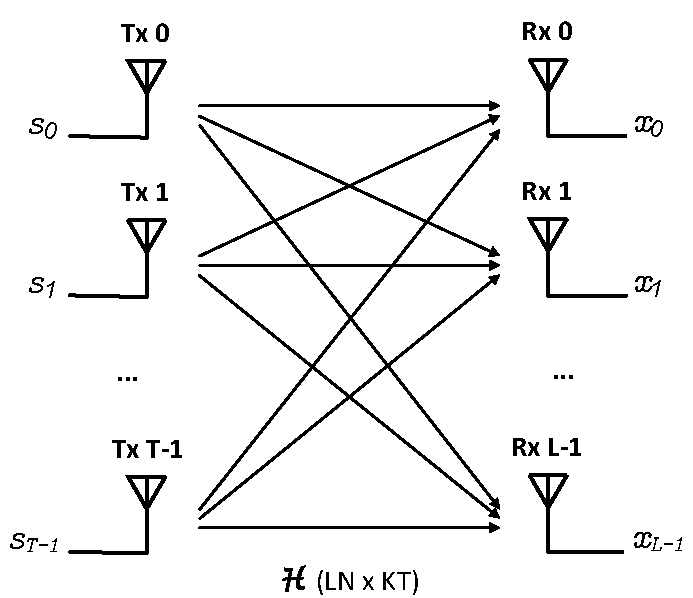
\includegraphics[width=0.6\linewidth]{figures/sys_model.pdf}
    \caption{Mô hình minh hoạ hệ thống truyền thông MIMO.}
    \label{fig:sys_model}
\end{figure}

Hình~\ref{fig:sys_model} minh hoạ một hệ thống thu phát MIMO/mMIMO, với $T$ ăng-ten phát và $L$ ăng-ten thu. Mỗi kênh truyền vô tuyến giữa ăng-ten phát thứ $t$ và ăng-ten nhận thứ $l$ sẽ được mô hình hoá bằng một bộ lọc đáp ứng xung hữu hạn (FIR - Finite impulse response) tương ứng là một véc-tơ của các hệ số bộ lọc có độ dài $M+1$. Giả sử ở mỗi thời điểm $i$, mỗi ăng-ten thu sẽ thu thập một chuỗi $N$ ký hiệu (symbol) liên tiếp. Từ các giả thiết trên, mô hình toán học của hệ thu phát MIMO được biểu diễn dưới dạng ma trận như sau

\begin{equation}
    \mathbf{x}(i) = \sum_{t=0}^{T-1}\mathbf{H}_t \mathbf{s}_t(i) + \mathbf{w}_t
\end{equation}
trong đó $\mathbf{s}_t(i) \in \mathbb{C}^{M+N \times 1}$ là các ký hiệu được gửi đi từ bộ phát thứ $t$. Ma trận kênh truyền dạng tích chập (convolution)~\cite{original} giữa bộ phát thứ $t$ và toàn bộ $L$ ăng-ten thu được ký hiệu $\mathbf{H}_t$. Giả sử rằng $\mathbf{H}_t \in \mathbb{C}^{LN \times K}$ là một ma trận đầy đủ hạng theo cột (full column rank) với hạng $K = M+N$. Tiếp đến, $\mathbf{x}(i) \in \mathbb{C}^{LN \times 1}$ là véc-tơ biểu diễn tín hiệu thu được từ $L$ ăng-ten. Cuối cùng, $\mathbf{w}_t \in \mathbb{C}^{LN \times 1}$ đại diện cho tạp âm trắng cộng sinh (AWGN - additive white Gaussian noise). Giả sử kênh truyền và tạp âm ở các kênh khác nhau là độc lập và phân bố giống nhau (i.i.d) với các phân bố lần lượt được chọn là $\mathcal{CN}(0, \sigma_{\mathbf{H}_t}^2 \mathbf{I})$ và $\mathcal{CN}(0, \sigma^2 \mathbf{I})$. Dưới đây là biểu diễn đầy đủ của các thành phần kể trên với $(.)^\top$ là phép chuyển vị (transpose) ma trận.

\begin{equation}
    \mathbf{s}_t(i) = [s(i), s(i-1),\ldots,s(i-K+1)]^\top
\end{equation}

\begin{equation}
    \small
    \mathbf{H}_t= \hspace{-0.7cm}
    \begin{array}{cc}
         & \underset{\longleftrightarrow}{K}\\
         & \left(\begin{array}{cccccc}
    h_0^{(0)} & \cdots & h_M^{(0)} & 0 & \cdots & 0 \\
    \vdots & \cdots & \ddots & \cdots & \ddots & 0 \\
    0 & \cdots & 0 & h_0^{(0)} & \cdots & h_M^{(0)} \\
    \vdots & \cdots & \vdots & \cdots & \cdots & \vdots \\
    h_0^{(L-1)} & \cdots & h_M^{(L-1)} & 0 & \cdots & 0 \\
    \vdots & \cdots & \ddots & \cdots & \ddots & 0 \\
    0 & \cdots & 0 & h_0^{(L-1)} & \cdots & h_M^{(L-1)}
    \end{array}
    \right) 
    \end{array}
    \Big\updownarrow LN    
\end{equation}

\begin{equation}
        \mathbf{x}(i) = \big[x^{(0)}(i), \cdots, x^{(0)}(i-N+1), \cdots, 
        x^{(L-1)}(i), \cdots, x^{(L-1)}(i-N+1)\big]^\top
\end{equation} 

Cần lưu ý rằng, cách biểu diễn toán học dưới dạng ma trận số phức như trên chỉ phù hợp trên lý thuyết và các phần mềm mô phỏng như Matlab. Các phương pháp sử dụng ML/DL nhằm nhận dạng kênh thường được phát triển trên ngôn ngữ Python và các thư viện nền tảng thông dụng như Tensorflow\footnote{\url{https://github.com/tensorflow/tensorflow}} của Google hay Pytorch\footnote{\url{https://github.com/pytorch/pytorch}} của Facebook, cả hai thư viện này không trực tiếp hỗ trợ các phép toán/toán tử với số phức. Do vậy, không làm mất đi tính tổng quát, ở chương~\ref{sec:ML}, các ma trận trên mô hình kênh kể trên sẽ được biểu diễn dưới dạng ma trận của các thành phần thực ($\Re$) và ảo ($\Im$) riêng biệt như sau

\begin{equation}
    \mathbf{s}_t=\left[\begin{array}{l}
    \Re(\mathbf{s}_t) \\
    \Im(\mathbf{s}_t)
    \end{array}\right] ;
    \mathbf{x}=\left[\begin{array}{l}
    \Re(\mathbf{x}) \\
    \Im(\mathbf{x})
    \end{array}\right] ; 
    \mathbf{w}_t=\left[\begin{array}{l}
    \Re(\mathbf{w}_t) \\
    \Im(\mathbf{w}_t)
    \end{array}\right]
\end{equation}

\begin{equation}
    \mathbf{H}_t=\left[\begin{array}{cc}
    \Re(\mathbf{H}_t) & -\Im(\mathbf{H}_t) \\
    \Im(\mathbf{H}_t) & \Re(\mathbf{H}_t)
    \end{array}\right]
\end{equation}

\section{Nhận dạng kênh không mù}
Như trên hình~\ref{fig:classify}, các phương pháp nhận dạng kênh không mù có thể chia làm hai nhóm chính, bao gồm các phương pháp sử dụng dữ liệu (Data-aided)~\cite{vilas2022} và các phương pháp dựa trên hướng quyết định (Decision-directed)~\cite{Ozdemir2007}. Các thuật toán sử dụng dữ liệu có thể chia làm hai loại nhỏ hơn, gồm có các phương pháp dựa trên việc đào tạo (Training-based) và các phương pháp dựa trên tín hiệu hoa tiêu (Pilot-assisted). Khác biệt chính giữa hai phương pháp là loại tín hiệu được dùng để ước lượng kênh truyền. Với Training-based, bên phát sẽ phát các dữ liệu huấn luyện gốc, bên thu chỉ biết thời điểm dữ liệu huấn luyện này được truyền nhưng không biết trước thông tin của dữ liệu. Tín hiệu bên thu nhận được gồm tín hiệu gốc và tín hiệu đã bị méo, từ đó, một mô hình ước lượng được huấn luyện bằng cách tối ưu hóa một hàm mất mát (loss function) giữa kết quả ước lượng kênh truyền và giá trị thực tế của kênh truyền. Với Pilot-assisted, các ký hiệu pilot được chèn trực tiếp vào khung dữ liệu gửi đi, và bên phát biết cả thời gian, vị trí, và giá trị gốc của các ký hiệu pilot này. Từ đó, bên thu có thể ước lượng ra ảnh hưởng của kênh truyền đến các tín hiệu pilot và nội suy ra ảnh hưởng của kênh truyền đến toàn bộ khung dữ liệu. Các giải thuật phổ biến được sử dụng cho phương pháp Data-aided có thể kể đến như bộ phát hiện ép về không (ZF - Zero Forcing), lỗi trung bình phương sai tối thiểu (MMSE - Minimum Mean Square Error)~\cite{Jiang2011}. Hai giải thuật này là các giải thuật tuyến tính và sẽ được trình bày chi tiết hơn ở mục~\ref{sec:zf} và~\ref{sec:mmse}. Tuy phổ biến và được áp dụng trong các hệ truyền thông thực tế, nhưng các phương pháp sử dụng dữ liệu để ước lượng kênh truyền có một nhược điểm đó là giảm hiệu quả sử dụng phổ do một phần băng thông bị lãng phí để truyền tải các dữ liệu huấn luyện hoặc pilot. 

Phương pháp hướng quyết định (DDCE - Decision-directed channel estimation) cũng dựa trên việc sử dụng dữ liệu, tuy nhiên, thay vì ước lượng kênh truyền chỉ trong một bước DDCE có thêm một bước nữa~\cite{vilas2022}. Cụ thể, tại bước một, DDCE vẫn ước lượng kênh truyền dựa trên một trong hai phương pháp Training-based hoặc Pilot-assisted như Data-aided. Sau đó, khôi phục các tín hiệu dựa trên trạng thái kênh truyền vừa ước lượng được. Ở bước tiếp theo, các dữ liệu mới được khôi phục sẽ tiếp tục được đưa vào thuật toán ước lượng nhằm cập nhật trạng thái thông tin về kênh truyền cho đến khi các ký hiệu trong một phiên được truyền hết. Chi tiết hơn, bộ thu sẽ so sánh ký tự đã nhận được với ký tự được dự đoán dựa trên ký tự trước đó và ước lượng kênh truyền hiện tại. Nếu có sai sót giữa ký tự đã nhận và ký tự dự đoán, bộ thu sẽ điều chỉnh ước lượng kênh truyền để cải thiện độ chính xác của dự đoán ký tự tiếp theo. Quá trình này được lặp lại cho mỗi ký tự nhận được. Vậy ra quyết định bít là 0 hay 1 trong DDCE sẽ được thực hiện theo hai giải thuật gồm quyết định mềm (soft) và quyết định cứng (hard). Quyết định mềm~\cite{Park2015} sẽ xác định giá trị của các bít dữ liệu bằng cách tính toán xác suất bit đó được truyền qua kênh truyền. Ngược lại, với quyết định cứng~\cite{Kai2005}, một ngưỡng xác định được đưa ra, nếu lớn hơn ngưỡng này sẽ là bít 1, ngược lại là bít 0. Tuy nhiên, phương pháp DDCE có điểm hạn chế đó là quá trình ước lượng lại bị phụ thuộc vào các dữ liệu cũ, dẫn đến việc, có thể kênh truyền hiện tại không còn tương ứng với các dữ liệu từ thời điểm quá khứ. Điều này dẫn đến các lỗi tích luỹ và làm giảm hiệu năng của hệ thống nhận dạng.

\subsection{Zero Forcing (ZF)} \label{sec:zf}

Các giải thuật nhận dạng tuyến tính dựa trên các phép biến đổi tuyến tính của các tính hiệu nhận được $\mathbf{x}$. Các giải thuật tuyến tính thường có độ phức tạp thấp, hoặc trung bình. Nhưng độ phức tạp sẽ tăng lên nếu hệ thống có số chiều lớn, ví dụ số lượng ăng-ten $T$ hay $L$ rất lớn trong mMIMO dẫn đến phép nghịch đảo ma trận tiêu tốn nhiều tài nguyên tính toán hơn. Một bộ nhận dạng tuyến tính có thể biểu diễn như bên dưới
\begin{equation}
    \mathbf{s} = \mathbf{G} \mathbf{x}
\end{equation}

ZF là phương pháp đơn giản nhất của các thuật toán nhận dạng tuyến tính. Trong đó, ma trận kênh truyền $\mathbf{H}$ sẽ được nghịch đảo để loại bỏ ảnh hưởng của kênh truyền. Ma trận làm bằng (equalizer matrix) $\mathbf{G}_{ZF}$ của bộ nhận dạng ZF như sau
\begin{equation}
    \mathbf{G}_{ZF}=\left(\mathbf{H}^H \mathbf{H}\right)^{-1} \mathbf{H}^H
\end{equation}
với $\mathbf{G}_{ZF}$, tín hiệu gốc được khôi phục bằng cách
\begin{equation}
    \hat{\mathbf{s}}_{ZF}=\left(\mathbf{H}^H \mathbf{H}\right)^{-1} \mathbf{H}^H \mathbf{x}
\end{equation}

\subsection{Minimum Mean Square Error (MMSE)} \label{sec:mmse}

Hiệu năng của bộ nhận dạng ZF thường bị ảnh hưởng bởi nhiễu AWGN. Do vậy, MMSE là giải thuật tốt hơn bằng việc kết hợp thêm thông tin phương sai của nhiễu trước khi nghịch đảo ma trận. Ma trận làm bằng $\mathbf{G}_{MMSE}$ của bộ nhận dạng MMSE được biểu diễn dưới dạng

\begin{equation}
    \mathbf{G}_{MMSE}=\left(\mathbf{H}^H \mathbf{H}+\frac{\sigma^2}{E_\mathbf{x}} \mathbf{I}\right)^{-1} \mathbf{H}^H
\end{equation}
với $\sigma^2$ là phương sai của nhiễu AWGN, $E_\mathbf{x}$ là công suất của tín hiệu thu được, và $\mathbf{I}$ là ma trận đơn vị. với $\mathbf{G}_{MMSE}$, tín hiệu gốc được khôi phục như sau
\begin{equation}
    \hat{\mathbf{s}}_{MMSE}=\left(\mathbf{H}^H \mathbf{H}+\frac{\sigma^2}{E_\mathbf{x}} \mathbf{I}\right)^{-1} \mathbf{H}^H \mathbf{x}
\end{equation}

Ưu điểm của MMSE, các giá trị thấp trong quá trình đảo ngược có thể dẫn đến hiện tượng khuếch đại tạp âm (deep null) khi sử dụng ZF, được khắc phục bởi công suất tạp âm khác không. Tuy nhiên, có thể nhận thấy cả hai giải thuật ZF và MMSE cần các chuỗi pilot để ước lượng kênh truyền, sau đó nội suy ra ma trận $\mathbf{H}$.
% \subsection{Maximum Likelihood Detector (MLD)}

\section{Nhận dạng kênh mù} \label{sec:blind}

Các kỹ thuật nhận dạng hệ thống mù (hoặc tương tự như giải mã mù hoặc cân bằng mù) đã được biết đến từ đầu những năm 1980. Theo~\cite{vilas2022}, có thể chia các thuật toán mù vào hai nhóm chính. Thứ nhất là các kỹ thuật ước lượng kênh truyền dựa trên đặc tính thông kê của tín hiệu thu được, có thể là đặc tính thống kê bậc hai (SOS - Second-order statistics), hoặc bậc cao (HOS - Higer-order statistics). Cách tiếp cận SOS được đề xuất trong~\cite{Tong1994} yêu cầu các tín hiệu có đặc tính chu kỳ hoặc đa dạng kênh (channel diversity) với các hệ thống đơn đầu đơn vào đầu ra (Single-input single-output). SOS có ưu điểm là yêu cầu lượng dữ liệu ít hơn để có được các ước tính thống kê đáng tin cậy tương đương với phương pháp HOS. Tuy nhiên, HOS~\cite{Giannakis1997} có lợi thế là cung cấp thông tin về pha mà không cần đa dạng kênh với đánh đổi là cần một lượng lớn dữ liệu lấy mẫu và khả năng tính toán cao hơn.

Nhóm kỹ thuật thứ hai đó là khai thác các thông tin đã xác định (deterministic) của tín hiệu hoặc hệ thống. Có thể kể đến như thuật toán mô-đun không đổi (CMA - Constant modulus algorithm)~\cite{Treichler1983} khai thác đặc trưng là giá trị mô-đun không đổi của các tín hiệu phức khi sử dụng các bộ điều chế như điều chế pha (PSK - Phase-shift keying), điều chế biên độ cầu phương 4 điểm (4-QAM - Quadrature amplitude modulation). Từ đó, nhóm tác giả đề xuất cân bằng kênh truyền bằng một bộ lọc thích nghi (adaptive filter) để đưa mô-đun của tín hiệu thu được về các giá trị chuẩn của PSK hay 4-QAM. Thuật toán MRE~\cite{original} khai thác đặc trưng tham chiếu của hệ thống gồm nhiều cảm biến thu (sensor) hay được hiểu là đa ăng-ten trong một hệ đơn đầu vào đa đầu ra (SIMO - Single-input multi-output). Nhóm tác giả đề xuất phương pháp ước lượng một tập $N$ bộ lọc để làm bằng kênh, tương ứng với $N$ mẫu độ trễ ở các ăng-ten khác nhau. Trong~\cite{Bey2011}, nhóm tác giả đặc trưng thưa (sparsity) của tín hiệu thường xuất hiện nhiều trong các kênh truyền mMIMO hay bước sóng mi-li-mét (mmWave - millimeter Wave) hiện nay. Bằng cách sử dụng tính chất thưa, các tín hiệu gốc có thể được khôi phục trong trường hợp hệ thống dưới mức xác định (underdeterminied). Trong một số điều kiện cụ thể, việc áp dụng ràng buộc thưa có thể làm cải thiện hiệu năng của việc nhận dạng hệ thống mù.

\section{Nhận dạng kênh bán mù} \label{sec:semi}

Các phương pháp nhận dạng kênh bán mù được sinh từ sự kết hợp của các kỹ thuật Non-blind (NB) và Blind. Giải pháp lai (hybrid) này được kỳ vọng sẽ giảm thiểu lượng pilot cần thiết mà vẫn bù đắp lại được độ chính xác bằng các thông tin từ kỹ thuật mù mang lại. Các tiếp cận đơn giản nhất đó là kết hợp trực tiếp các bộ nhận dạng như ZF, MMSE với các thông tin thống kê SOS, HOS đã được trình bày ở trên. Các công bố~\cite{Wan2008, Ladaycia2019, Rekik2021} đi theo hướng tiếp cận này đều cho ra các kết quả vượt trội khi so với với NB truyền thống trong một số điều kiện nhất định. Ngoài ra, việc kết hợp các thông tin xác định của các bộ cân bằng mù như được trình bày ở mục~\ref{sec:blind} cũng là các hướng nghiên cứu tiềm năng trong tương lai.

Tiếp đến, ngoài các đặc trưng của tín hiệu, các thông tin bên lề (side-information) của hệ thống thu phát cũng có thể được xem xét để cải thiện khả năng nhận dạng kênh truyền. Có thể kể đến như sử dụng thêm thông tin hướng sóng đến/đi (DoA/DoD) như trong~\cite{Wang2016}, nhóm tác giả đã đề xuất sử dụng DoA của các người dùng khác nhau để giảm thiểu/loại bỏ sự ảnh hưởng của ô nhiễm pilot (PC - Pilot contamination) qua đó hiệu suất của việc nhận dạng kênh truyền đã được cải thiện. Tiếp đến,~\cite{Lin2020} đề xuất sử dụng thông tin về toạ độ/vị trí (location) người dùng để đánh giá đáp ứng tần số kênh truyền mmWave. Kết quả mô phỏng cho thấp cả độ chính xác và độ phức tạp của mô hình ước lượng đều giảm đi khi có thêm loại thông tin bên lề này.

\section{Nhận dạng kênh sử dụng học máy}

Nhận dạng kênh truyền sử dụng ML/DL là hướng tiếp cận bùng nổ trong các năm trở lại đây. Do các bước tiến đã đạt được trước đó của việc xử lý các loại tín hiệu âm thanh, hình ảnh sử dụng các mạng học sâu. Việc chuyển tiếp các kỹ thuật sẵn có này sang viễn thông được xảy ra nhanh chóng và bước đầu các nghiên cứu đã chỉ ra các kết quả tiềm năng. Điểm khác biệt của hướng tiếp cận này đó là nó bao hàm được lý thuyết của cả ba hướng tiếp cận kể trên bao gồm mù, bán mù, và không mù. Tuy nhiên, thay vì việc tìm các phương pháp tối ưu và nghiệm chính xác, ML/DL sử dụng các thuật toán ML cơ bản, mạng nơ-ron (NN - Neuron network), hay học tăng cường (RL - Reinforcement learning) cho các đầu vào của hệ thống nhận dạng B, SB, NB.

Các phương pháp sử dụng học cổ điển để nhận dạng kênh truyền được phát triển trước tiên, do độ phức tạp ở mức thấp. Trong~\cite{Simeon2022}, việc ước lượng ma trận làm bằng $\mathbf{G}_{MMSE}$ được thay thế bằng thuật toán hồi quy Gaussian (GPR - Gaussian process regression). Các ưu điểm của GPR như tỷ (i) lệ lỗi bít (BER - Bit error rate) thấp hơn MMSE truyền thống; (ii) nội suy chính xác hơn các ước tính kênh ở giữa các pilot symbol so với các kỹ thuật nội suy tuyến tính. Ngoài phương pháp hồi quy, các giải thuật cổ điển của học máy như giảm số chiều của dữ liệu (PCA - Principal components analysis, ICA - Independent component analysis), học Bayesian cũng được đề xuất và cho thấy sự hiệu quả~\cite{vilas2022}.

Các phương pháp nhận dạng sử dụng các mạng nơ-rơn còn có những bước tiến rõ ràng hơn, khi NN phức tạp hơn và số lượng tham số đào tạo cũng là rất lớn để đáp ứng được các mô hình kênh phức tạp. Các nghiên cứu trong mục~\ref{sec:semi} như~\cite{Lin2020, Wan2008} cũng sử dụng các thông tin bên lề cho SB nhưng thay vì các phương pháp tối ưu, các mạng nơ-ron sâu (DNN - Deep-neural network) đã được đề xuất đề ước lượng kênh truyền. Một trong những mạng DNN đầu tiên được đề xuất cho việc nhận dạng hệ thống MIMO đó là mạng phát hiện (DetNet - Detection network)~\cite{Samuel2019}. Với kiến trúc là các phép lặp của thuật toán giảm độ dốc dự kiến kết (gradient descent) hợp thành một mạng. DetNet đã cho kết quả về độ chính xác vượt trội các phương pháp nhận dạng tuyến tính ở mức BER đạt $10^-3$~dB tại tỷ số tín trên tạp (SNR - Signal noise ratio) $10$~dB. Tuy nhiên, do số lượng tham số cần đào tạo là lớn nên quá trình đào tạo có thể tốn chi phí, từ đó một số mạng ISD đã được đề xuất~\cite{Mandloi2017, Liao2020}, với độ chính xác tốt hơn DetNet nhưng số lượng tham số đào tạo chỉ dưới 100. Ngoài ra, rất nhiều các mô hình mạng NN khác đã được đề xuất, như mạng trí nhớ ngắn hạn định hướng dài hạn  (LSTM - Long/short-terrn memory), bộ tự mã hoá (Autoencoders),~\ldots~\cite{vilas2022}.

Tương tự như hai phương pháp kể trên, RL cũng được đưa sang ứng dụng cho nhận dạng kênh truyền. Trong nghiên cứu~\cite{Oh2021}, nhóm các tác giả đã trình bày một phương pháp khử nhiễu trên miền tần số dựa trên RL không cần kiến thức kênh tiền nghiệm và dữ liệu được dán nhãn trước. Cụ thể, thuật toán cung cấp một cải tiến đáng kể so với phương pháp ước lượng bình phương nhỏ nhất thực tế (LS - Least square) và mang lại hiệu suất tiệm cận với ước lượng lỗi bình phương trung bình nhỏ nhất tuyến tính (LMMSE - Linear MMSE) lý tưởng với toàn bộ thông tin về trạng thái kênh (CSI - Channel state information).